\model{Deck of Cards}

There are 52 cards in a standard deck.
Each card belongs to one of four suits (Clubs, Spades, Hearts, and Diamonds) and one of 13 ranks (Ace, 2, 3, 4, 5, 6, 7, 8, 9, 10, Jack, Queen, and King).
The array below is one-dimensional, but the cards are displayed on four lines for convenience.

\begin{center}
% http://www.milefoot.com/math/discrete/counting/cardfreq.htm
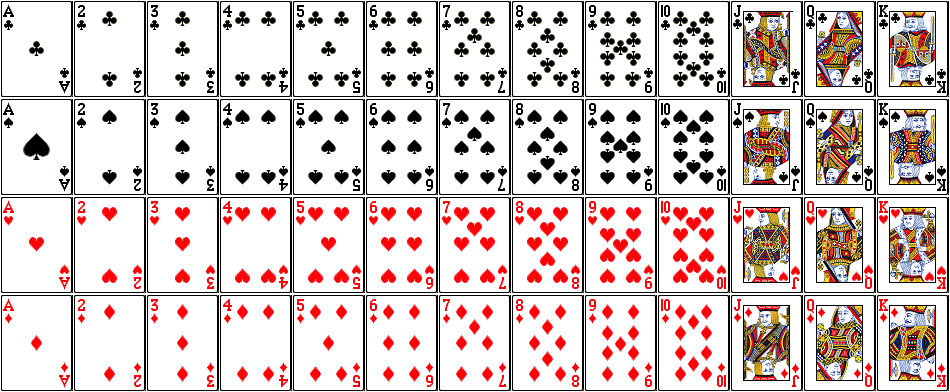
\includegraphics[width=\linewidth]{playing-cards1.png}
\end{center}


\quest{25 min}


\Q \label{cnstr}
Implement the following constructor.
The class has two attributes: \java{rank} and \java{suit}.
%You may assume the arguments are valid (rank is between 1 and 13, and suit is one of the four strings).
Make sure the arguments are within range, and if not, replace them with the minimum value.

\begin{javalst}
/**
 * Constructs a face card given its rank and suit.
 *
 * @param rank face value (1 = ace, 11 = jack, 12 = queen, 13 = king)
 * @param suit category (0 = clubs, 1 = diamonds, 2 = hearts, 3 = spades)
 */
public Card(int rank, int suit) {
\end{javalst}

\vspace*{-1em}
\begin{answer}[14em]
\begin{javaans}
    if (rank < 1 || rank > 13) {
        this.rank = 1;
    } else {
        this.rank = rank;
    }

    if (suit < 0 || suit > 3} {
        this.suit = 0;
    } else {
        this.suit = suit;
    }
\end{javaans}
\end{answer}
\vspace*{-1em}

\begin{javalst}
}
\end{javalst}


\Q In one line of code, declare an array of \java{int}s named \java{suits} and initialize its contents to the four possible suits as shown in \ref{\currfilename}.

%   String[] suits = {"clubs", "spades", "hearts", "diamonds"};

\vspace*{-1ex}
\begin{answer}[3em]
\begin{javaans}
    int[] suits = {0, 3, 2, 1};
\end{javaans}
\end{answer}


\Q \label{build}
Write several lines of code to declare and create an array of 52 \java{Card} objects.
Use nested \java{for} loops to construct \java{Card} objects in the order of \ref{\currfilename}.
Make use of your \java{suits} array from the previous question.
Discuss with your team how you will keep track of the array index.

\vspace*{-1ex}
\begin{answer}[11em]
\begin{javaans}
Card[] cards = new Card[52];
int index = 0;
for (int suit : suits) {
    for (int rank = 1; rank <= 13; rank++) {
        cards[index] = new Card(rank, suit);
        index++;
    }
}
\end{javaans}
\end{answer}


\Q If you did not use an enhanced for loop in the previous question, go back and simplify your answer.
Explain why an enhanced for loop is appropriate for one of the variables (suit or rank) but not the other.

\begin{answer}[5em]
Because the suits are out of order, we rely on the \java{suits} array to determine how to create the cards.
It's easier to pull values out of an array with an enhanced for loop.
The rank values simply iterate from 1 to 13 in order, so a standard for loop is appropriate for that task.
\end{answer}


\Q Describe what the following code does and how it works. (Note: You've come a long way this semester, to be able to understand this example!)

\begin{javalst}
public static Card[] sort(Card[] deck) {
    if (deck == null) {
        System.err.println("Missing deck!");
        return null;
    }
    Card[] sorted = new Card[deck.length];
    for (Card card : deck) {
        int index = card.position();       // returns suit * 13 + rank - 1
        sorted[index] = card;
    }
    return sorted;
}
\end{javalst}

\begin{answer}[5em]
This example sorts an array of cards.
It first validates the arguments, then it creates a new array of cards and assigns each \java{Card} reference according to its known position in the deck.
\end{answer}


\Q Identify examples of the following Java language features in the previous question.
\begin{enumerate}
\item variables \ans{deck, sorted, card, index}
\item decisions \ans{if (deck == null)}
\item loops \ans{for (Card card : deck)}
\item methods \ans{sort, println, position}
\item arrays \ans{deck, sorted}
\item objects \ans{"Missing deck!", card}
\end{enumerate}



\Q \label{search}
Write a static method named \java{inDeck} that takes a \java{Card[]} representing a deck of cards and a \java{Card} object representing a single card, and that returns \java{true} if the card is somewhere in the deck of cards. Be sure to use the equals method of the \java{Card} object to make comparisons.

\vspace{-1ex}
\begin{answer}[11em]
\begin{javaans}
public static boolean inDeck(Card[] deck, Card card) {
    for (Card c : deck) {
        if (c.equals(card)) {
            return true;
        }
    }
    return false;
}
\end{javaans}
\end{answer}
